\chapter{場景建立}
\section{前言}
因為這次老師重新規劃了球場及球員的大小、重量......等等,我們重新規劃了整個球場及新建了球員模型,沒有沿用過去的設計。\\
\section{建立球員}
我們使用Onshape重新繪製了球員模型,這次規劃想改變過去bubbleRob看起來較呆版,圓潤的設計,因此設計了一台跑車作為我們的球員。File-Import-Mesh,選擇要匯入的檔案匯入球場,如(圖.\ref{球員建立}) 。接著加入joint\\
加入joint:滑鼠右鍵-Add-Joint-Revolute\\
\
\begin{figure}[hbt!]
\begin{center}
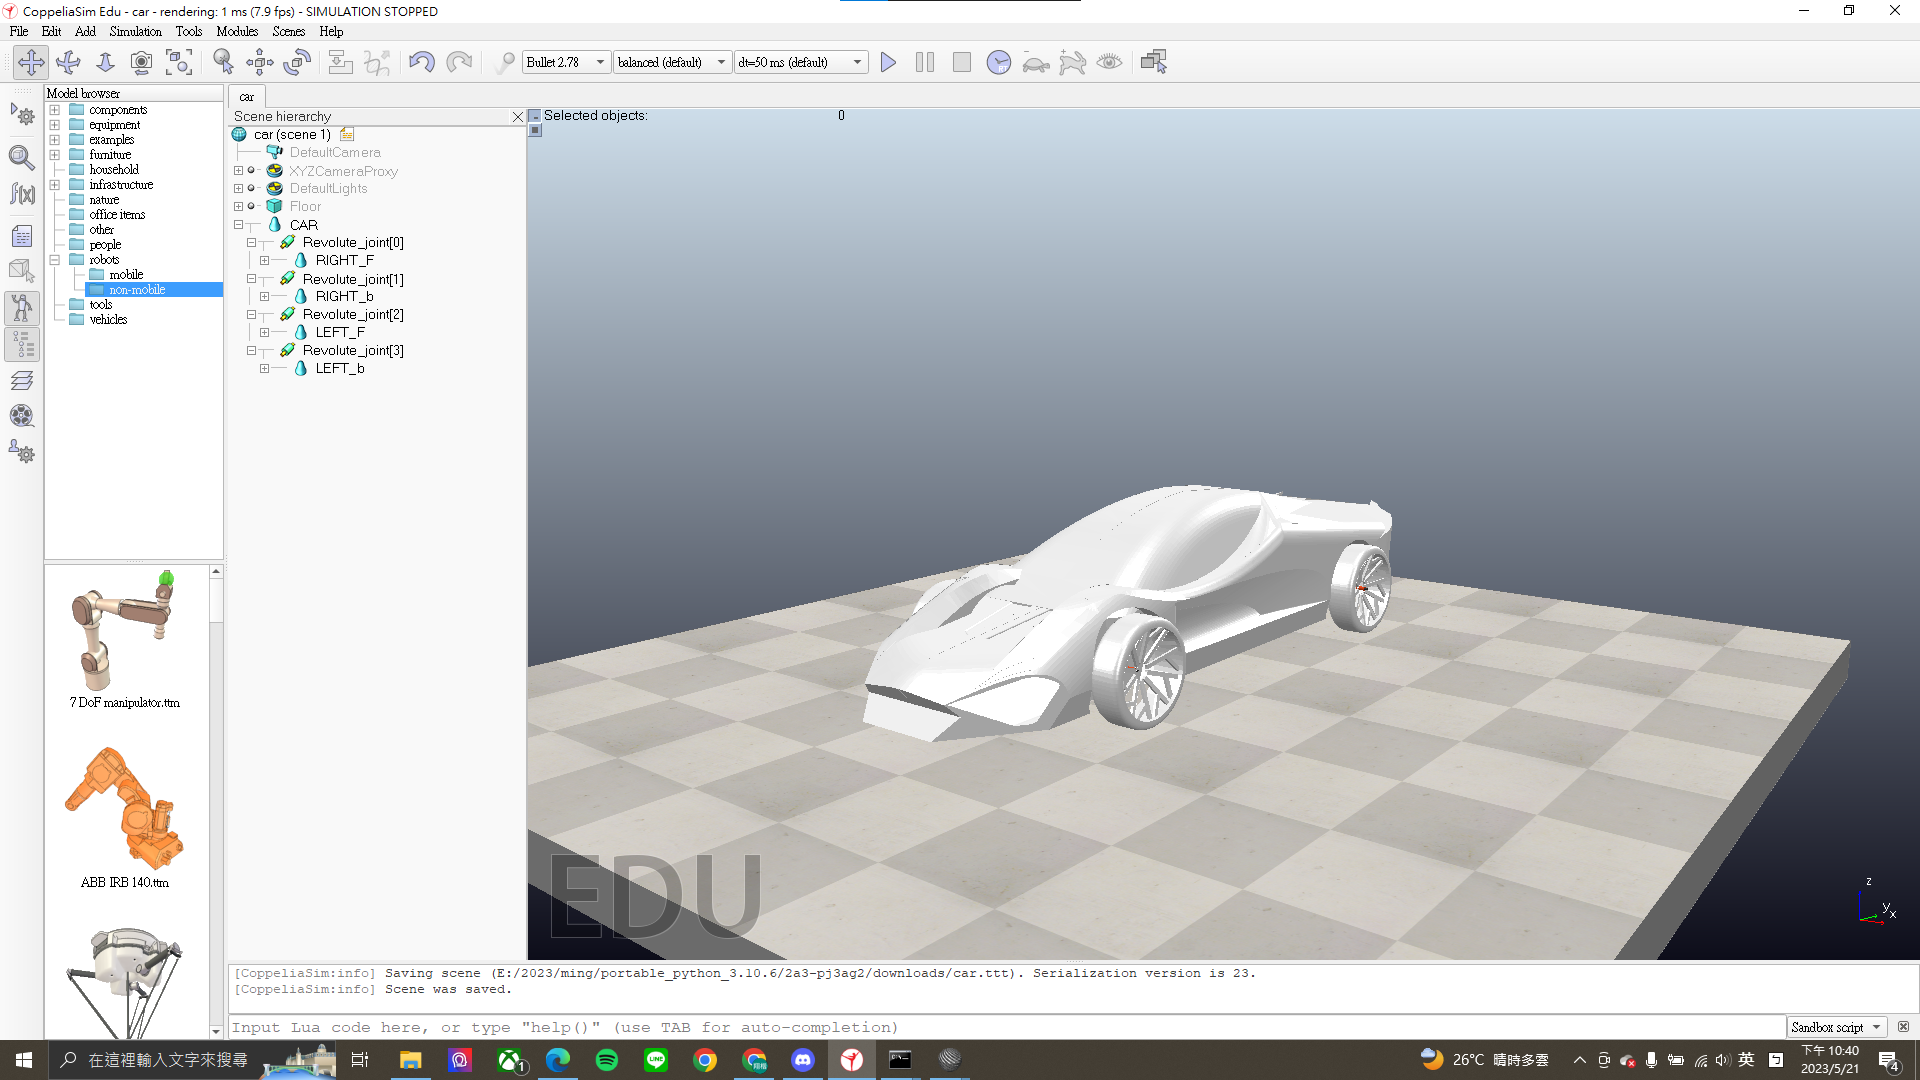
\includegraphics[width=12cm]{球員}
\caption{\Large 球員建立}\label{球員建立}
\end{center}
\end{figure}
\\
\
後發現比例錯誤,因此直接在CoppeliaSim內進行縮小,但因本來設計的跑車高度太低太扁平,可能會有無法推到球的狀況發生,因此不是使用等比縮小,而是直接將各部分拉至規定尺寸。如(圖.\ref{球員建立2})\\
\
比例放大縮小步驟:點選物件左邊圖示-View modify geornrtry-若勾選Keep proportions為進行等比放大,若取消勾選擇可以個別調整大小。\
\begin{figure}[hbt!]
\begin{center}
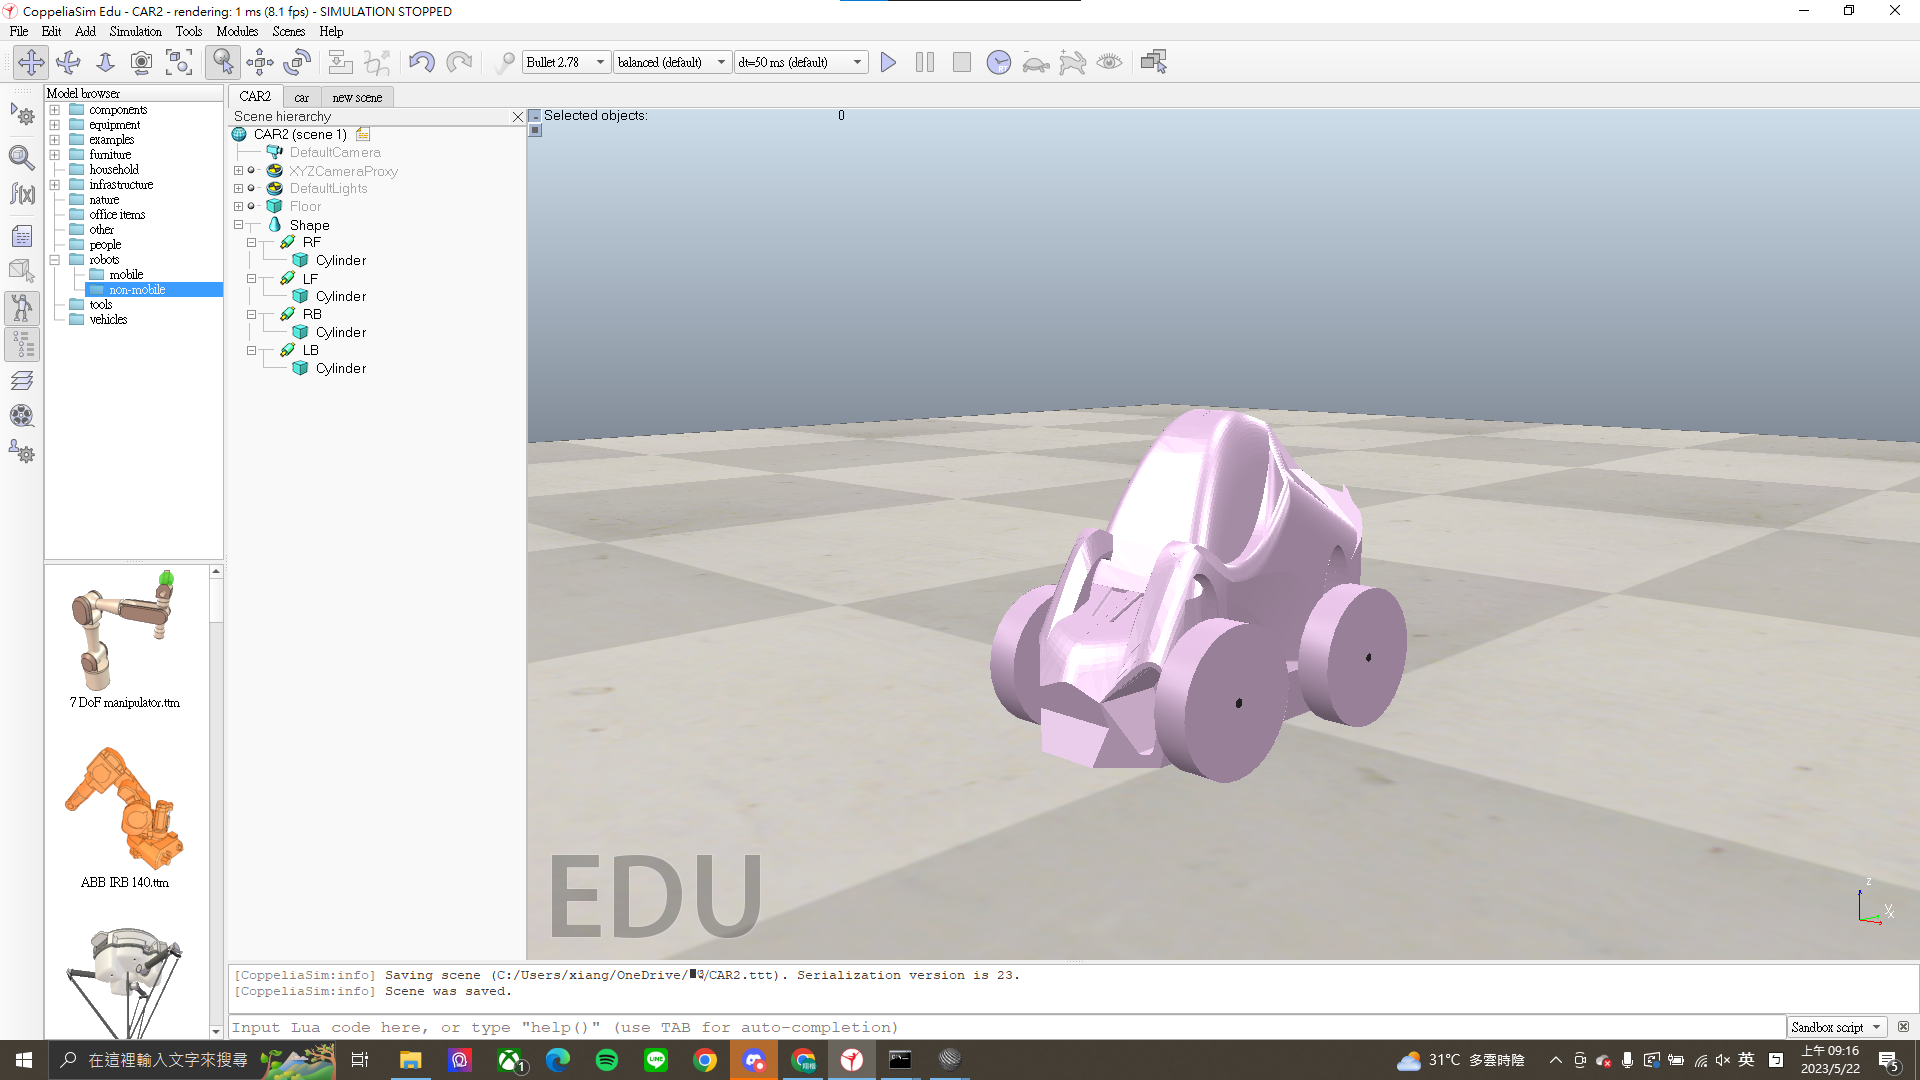
\includegraphics[width=12cm]{球員2}
\caption{\Large 球員建立2}\label{球員建立2}
\end{center}
\end{figure}\